\documentclass[12pt]{article}

% --- Packages ---
\usepackage{graphicx}  % include images
\usepackage{float}     % for [H] placement
\usepackage{caption}   % nicer captions
\usepackage{fancyhdr}  % headers and footers

% --- Header setup ---
\pagestyle{fancy}
\fancyhead[L]{Zeshui Song}       % left header
\fancyhead[R]{Ph291--Section E}     % center header        
\fancyfoot[C]{\thepage}          % page number in the footer
\setlength{\headheight}{15pt}


\renewcommand{\headrulewidth}{0.4pt} % header line thickness
\renewcommand{\footrulewidth}{0pt}   % remove footer line
\begin{document}

\section*{Selfie}
\textbf{Inverted and enlarged scan of photo:}
\begin{figure}[H]
  \centering
  \includegraphics[width=0.45\textwidth]{selfie inv.PNG}
  \caption{A selfie captured with a pinhole camera. The camera previously suffered from significant light leaks at the corners, but after sealing the edges with additional tape and keeping it covered until exposure, the issue was greatly reduced.}
\end{figure}
\textbf{Initial photo with light leaks:}
\begin{figure}[H]
  \centering
  \includegraphics[width=0.45\textwidth]{bad selfie.PNG}
  \caption{The first photo taken with significant light leaks.}
\end{figure}
\newpage
\section*{Negatives of Selfie Photos:}
\newpage
\section*{Physical Principle}
\textbf{Inverted and enlarged scan of photo:}
\begin{figure}[H]
  \centering
  \includegraphics[width=0.5\textwidth]{boat.PNG}
  \caption{A pinhole photograph of the boat LILAC, docked at Pier 25 in Hudson River Park. This photo illustrates the physical principle of buoyancy as it floats above the water. Some blurriness is visible due to the boat’s motion during the long exposure.}
\end{figure}
\textbf{Original negative of photo:}
\newpage 
\section*{Alternate Developer}
\begin{figure}[H]
  \centering
  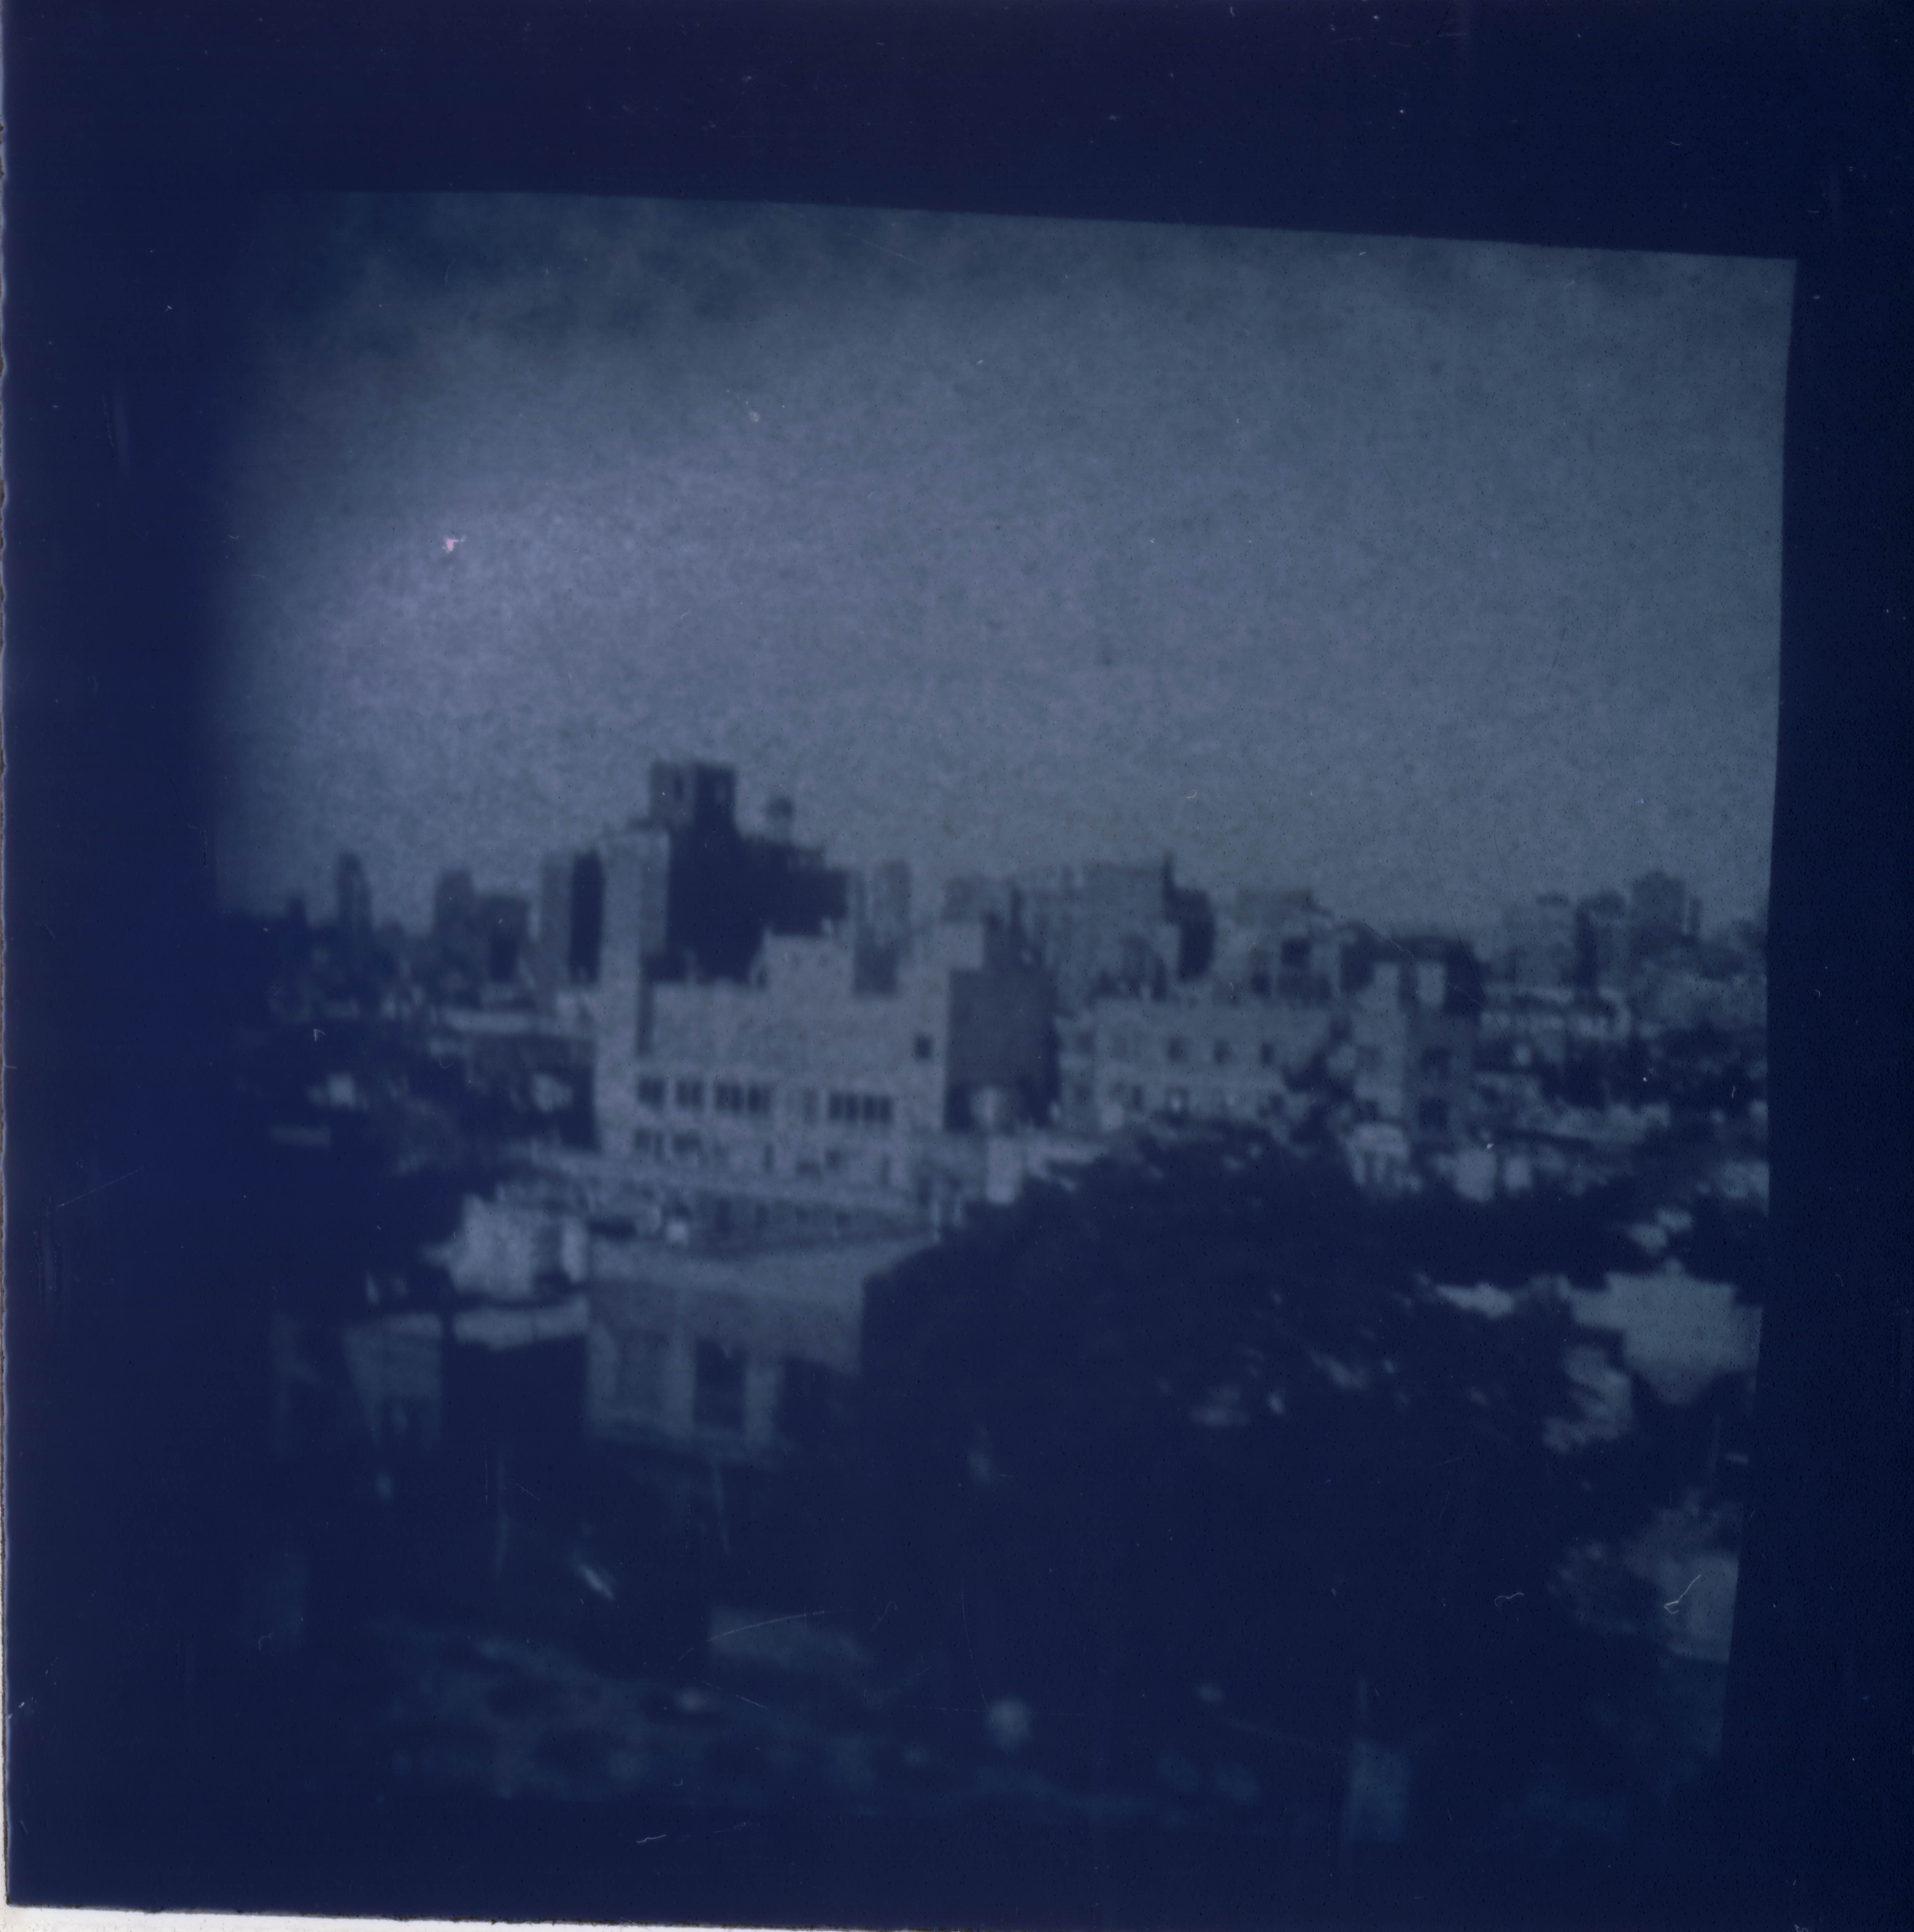
\includegraphics[width=0.5\textwidth]{alt.PNG}
  \caption{A pinhole photograph taken from the 8th-floor balcony. An alternative developer was used, prepared by mixing 400 mL of warm water with 4 teaspoons of washing soda, followed by 2 tablespoons of instant coffee and 1/2 teaspoon of vitamin C.}
\end{figure}
\textbf{Original negative of photo:}
\end{document}

